\begin{frame}

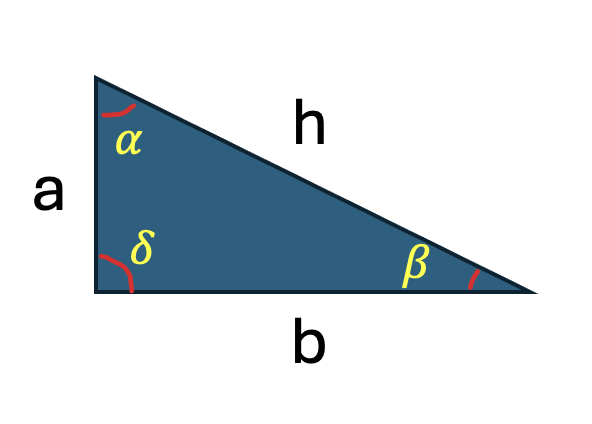
\includegraphics[scale=.3]{trian}

Este es un triángulo rectángulo y se cumple las siguientes relaciones:
 
\begin{enumerate}
\item $a^2 + b^2 = h^2$. Teorema de Pitagoras
\item $\sin \beta = \frac{a}{h}, \sin \alpha = \frac{b}{h}, \cos \beta = \frac{b}{h}, \cos \alpha = 
\frac{a}{h}, \tan \alpha = \frac{b}{a}$
\item $\sin^2 \theta + \cos^2 \theta = 1$
\item $\csc \alpha = \frac{1}{\sin \alpha}, \sec \alpha = \frac{1}{\cos \alpha}, \tan \alpha = \frac{\sin 
\alpha}{\cos \alpha}$
\end{enumerate}
\end{frame}


